\documentclass{article}
\usepackage{polski}
\usepackage[utf8]{inputenc}
\usepackage{hyperref}
\usepackage{graphicx}
\hypersetup{
    colorlinks,
    citecolor=black,
    filecolor=black,
    linkcolor=black,
    urlcolor=black
}

\title{Tworzenie projektu Open Source (Creating an Open Source project)}
\author{Mateusz Tylka}
\date{22 Listopada, 2021r}

\begin{document}

\maketitle
\newpage
\newpage
\tableofcontents
\newpage

\section{Wstęp}

\hspace{4mm} W naszym życiu codziennym napotykamy przeróżne systemy informatyczne. Korzystamy z nich posługując się urządzeniami cyfrowymi takimi jak komputer czy telefon komórkowy. Są to podstawowe narzędzia naszych czasów, bez których osoby fizyczne oraz firmy nie mogłyby prawidłowo funkcjonować.

Posługując się współczesnymi komputerami wykorzystujemy również odpowiednie oprogramowanie\footnote{\, Wymiennie będę stosował terminy: \emph{oprogramowanie, system informatyczny, program, program komputerowy, program informatyczny, aplikacja}} (ang. \emph{software}). Termin software oznacza zbiór instrukcji, które kierują pracą komputera w celu wykonania określonej czynności\cite{Kotula}. Wspomniany zbiór instrukcji jest zapisany w postaci kodu źródłowego (ang. \emph{source code}), który jest sporządzany przez programistów posługując się językami programowania. Można następująco zdefiniować: „\emph{kod źródłowy} (również \emph{źródło} lub \emph{źródła}) – program komputerowy w postaci takiej, jaką tworzy ją człowiek w pewnym języku programowania, zazwyczaj jako tekst, ale też jako dane dla translatora, przeznaczony do analizowania i modyfikacji przez człowieka. Kod źródłowy jest przetwarzany przez translator na kod maszynowy zrozumiały dla maszyny (procesora) lub jest analizowany i  wykonywany przez specjalny program zwany interpreterem, może być też przetworzony na kod pośredni”\cite{Kotula}. Ujmując to prościej: kod źródłowy można porównać do przepisu na potrawę kulinarną, gdzie tą potrawą w naszym przypadku jest program komputerowy. Posiadając przepis na daną potrawę, jesteśmy w stanie go modyfikować według naszych potrzeb, tworząc tym samym nowe dania. Czy jest również tak w przypadku programów informatycznych? 

Na początku, w latach 60. oraz 70. XX wieku pisanie oprogramowania było domeną małej grupy naukowców, którzy rozpowszechniali i udostępniali kod źródłowy w kręgach zainteresowanych osób. Tajniki tego zagadnienia były zatem dostępne, jednak pojawiła się chęć uznania własności oraz uzyskania zarobku. W tym samym czasie w branży komputerowej zaczęto zaprzestawać dostarczania kodu źródłowego wraz z oprogramowaniem, co miało zapewnić firmom wzrost zysków poprzez rozdzielną sprzedaż tych komponentów. W latach 60 rozpoczęto rejestrowanie programów komputerowych w urzędzie ochrony praw autorskich\cite{Kotula}. Na początku lat 70 programiści stopniowo zaczęli zarabiać pieniądze na podstawie własnych programów komputerowych, których kod źródłowy traktowali jako pilnie strzeżoną tajemnicę\cite{Richter}. Tak narodziło się oprogramowanie komercyjne, które rozpoczęło swoją intensywną ekspansję w latach 80\cite{Kotula}.

Pomimo komercjalizacji systemów informatycznych, były takie osoby jak Richard Matthew Stallman, których poglądy nie godziły się z koniecznością tworzenia oprogramowania zamkniętego (ang. \emph{closed source} - dostępnego w postaci kodu wykonywalnego). Zdanie Stallmana zostało ukształtowane przede wszystkim przez codzienną rzeczywistość pracy za pomocą urządzeń takich jak drukarka, której oprogramowanie było licencjonowane tak, że nie można było go przeprogramować, dostosowując do własnych potrzeb. „Konsument, nabywając jakiś produkt – taki jak drukarka laserowa – powinien mieć możliwość wykorzystania go w dowolny sposób”\cite{Kotula}. Stanowisko takich ludzi jak Stallman oraz wciąż pojawiająca się potrzeba na istnienie oprogramowania z dostępnym kodem źródłowym, doprowadziło do ukształtowania technologii określanych terminem \emph{open source}\footnote{\, Wymiennie będę stosował terminy: \emph{open source}, \emph{open source software}, \emph{oprogramowanie open source}, \emph{otwarte oprogramowanie} oraz akronimy \emph{OS}, \emph{OSS}.}. Początkowo przyjmowane w sposób niejednoznaczny, dziś zyskują coraz większą popularność i są coraz szerzej wykorzystywane\cite{Kotula}. 

Niniejsza praca poświęcona jest projektom oraz aspektom związanych z \emph{open source}. Praca składa się ze wstępu, bibliografii i trzech zasadniczych części. W pierwszym rozdziale zdefiniuję termin \emph{open source} oraz pojęcia z nim skorelowane, wymienię i opiszę kluczowe rodzaje licencji oraz porównam oprogramowanie otwarte z oprogramowaniem komercyjnym przywołując ich wady i zalety. Następnie wyjaśnię czym jest idea wolnego oprogramowania zwracając uwagę na jej różnice względem ruchu \emph{open source}. Przeanalizuje również kilka konkretnych przykładów otwartego oprogramowania w kontekście wolności i otwartości. W ostatniej części pracy opowiem o tworzeniu aplikacji \emph{open source} na podstawie projektu inżynierskiego \emph{Wmi Adventure}. Uzasadnię skąd wybór tego rodzaju licencji, jakie należy załączyć pliki oraz jaką dokumentację sporządzić do repozytorium\footnote{\, Miejsce, w których przechowuje się kod źródłowy oprogramowania.} projektowego. Wreszcie przedstawie ideę \emph{open source} w znaczeniu społecznym odwołując się do naszego projektu inżynierskiego.

\section{Definicja open source}

\hspace{4mm} W 1997 roku utworzony został i wprowadzony termin \emph{open source}. Twórcami tej koncepcji była pewna grupa osób, m.in. Eric S. Raymond, Tim O'Reilly i Bruce Perens. Ważnym elementem powstania tej idei był esej Reymonda pt. \emph{The cathedra and the bazaar} (pol. \emph{Katedra i bazar}), gdzie poruszył kwestię stylu rozwoju oprogramowania jaki prowadził Linus Torvarlds wraz z projektem systemu operacyjnego Linux. Reymond porównał ten proces do formy "hałaśliwego bazaru", gdzie wszyscy od samego początku projektu wprowadzali modyfikacje i proponowali własne rozwiązania\cite{Kotula}.  


W 1998 roku Eric Raymond i Bruce Perens powołali organizację non profit - \emph{Open Source Initiative} (skrót \emph{OSI})\cite{Kotula}. \emph{OSI} nadzoruje standard \emph{open source} (ang. \emph{The Open Source Definiction, OSD}), który jest używany do tego, aby jednoznacznie określać, czy dane oprogramowanie jest oprogramowaniem \emph{open source}. \emph{OSI} certyfikuje także licencje (\emph{OSI Certified}), aby potwierdzić, że dana
licencja spełnia postulaty \emph{OSD}\cite{opensource.org}. Pojęcie \emph{open source} jest zdefiniowane następującymi postulatami\cite{Kotula}:

\begin{enumerate}
    \item \textbf{Wolna redystrybucja (ang. \emph{free redistribution}).}
    
    \hspace{4mm} Brak zakazu sprzedawania lub rozdawania programu jako elementu większej całości, ani wymagania przekazywania określonych opłat ze sprzedaży. Można zatem wziąć kod źródłowy i wykorzystać go jako część większej aplikacji, a następnie dzieło sprzedać lub przekazać za darmo. Nie istnieje obowiązek uregulowania płatności za wcześniej wykorzystany fragment kodu lub cały kod źródłowy.
    
    \item \textbf{Kod źródłowy (ang. \emph{source code}).}
    
    \hspace{4mm} Takie oprogramowanie musi zawierać kod źródłowy, który jest rozpowszechniany zarówno w swojej pierwotnej postaci jak i w postaci skompilowanej (program gotowy do pracy). Kod źródłowy musi być dodatkowo dostępny w najprostszej postaci, aby była możliwość łatwego dokonywania w nim modyfikacji. Nie można celowo komplikować kodu źródłowego.
    
    \item \textbf{Dzieła pochodne (ang. \emph{derived works}).}
    
    \hspace{4mm} Licencja zgodna ze standardem \emph{OSD} musi zapewniać możliwość modyfikowania pierwotnego programu oraz tworzenia nowych aplikacji na jego bazie.
    
    \item \textbf{Spójność kodu źródłowego autora (ang. \emph{integrity of the author’s source code}).}
    
    \hspace{4mm} Licencja ma prawo zabraniać rozpowszechniania kodu źródłowego programu w zmodyfikowanej jego wersji tylko wtedy, gdy dozwolona jest dystrybucja poprawek do programu (ang. \emph{patch}) wraz z kodem źródłowym w celu ulepszania tego oprogramowania. Może też nakazywać, aby utwory pochodne posiadały inną nazwę oraz inny numer wersji niż program pierwotny. Dozwolony jest więc taki program, którego kod jest dostępny i dostępne są oddzielne poprawki, czyli \emph{patche}. Ten zapis zapewnia, że oryginalne prace pozostaną niezależnymi produktami.
    
    \item \textbf{Bez dyskryminacji osób i grup (ang. \emph{no discrimination against persons or groups}).}
    
    \hspace{4mm} Licencja nie może dyskryminować żadnych osób lub grup społecznych.
    
    \item \textbf{Bez dyskryminacji obszarów zastosowań (ang. \emph{no discrimination against fields of endeavor}).}
    
    \hspace{4mm} Oprogramowanie nie może być ograniczane co do wykorzystywania w dowolnym obszarze.
    
    \item \textbf{Dystrybucja licencji (ang. \emph{distribution of license}).}
    
    \hspace{4mm} Licencja nałożona na program jest jedynym przepisem prawnym, który obowiązuje taką aplikację. Na mocy tego zapisu następnym deweloperom nakazuje się stosowanie do tej regulacji. Innymi słowy dany program OS lub fragment kodu pozostaje na tej samej licencji w kolejnych wersjach i modyfikacjach.
    
    \item \textbf{Licencja nie może być przeznaczona dla konkretnego produktu (ang. \emph{license must not be specific to a product}).}
    
    \hspace{4mm} Wszystkie części danego programu open source muszą być udostępnione na prawach tej samej licencji. Punkt ten zapobiega opcji wyizolowania z danego OSS fragmentu kodu i publikacji go na innej licencji niż ta, która była przypisana danemu OSS.
    
    \item \textbf{Licencja nie może ograniczać innego oprogramowania (ang. \emph{license must not restrict other software}).}
    
    \hspace{4mm} Licencja nie może narzucać konieczności stosowania tych samych praw wobec całego systemu informatycznego, który jest dystrybuowany wraz z OSS. Innymi słowy, nie można nakazywać, aby rozpowszechniając dany program OSS na konkretnym urządzeniu, wszystkie inne aplikacje umieszczone na tym samym nośniku były również udostępniane na tej samej licencji. Zapis ten umożliwia wraz z oprogramowaniem komercyjnym swobodne rozpowszechnianie oprogramowania open source.
    
    \item \textbf{Licencja musi być neutralna technologicznie (ang. \emph{license must be technology-neutral}).}
    
    \hspace{4mm} Zapis ten powstał po to, aby pozwolić przenosić kod programu na inne nośniki, na przykład do postaci papierowej.
\end{enumerate}

Najprościej rzecz ujmując, idea open source polega na prowadzeniu oprogramowania, z otwartym kodem źródłowym, który można dowolnie kopiować, modyfikować oraz wykorzystywać do różnych celów. Jednak poszczególne aspekty zależą od danej licencji, na mocy której wytwarzane jest oprogramowanie. Omawiając specyficzne przypadki projektów open source będę odwoływał się do przedstawionej powyżej definicji w pozostałych częściach pracy.

\subsection{Rodzaje licencji}

\hspace{4mm} Licencja oprogramowania jest to umowa na korzystanie z utworu, jakim jest program komputerowy, zawierana pomiędzy podmiotem, któremu przysługują prawa autorskie do dzieła, a użytkownikiem, który zamierza z danej aplikacji korzystać\cite{wikipedia1}. Systemy informatyczne z otwartym kodem źródłowym posiadają wiele różnorodnych licencji. Potrzebują ich m.in. po to, aby umożliwiać dystrybucje oraz dostęp. Na mocy stosowanych licencji określone sytuacje stają się klarowne. 

Pierwszą licencją powiązaną z koncepcją otwartego kodu źródłowego była zaproponowana przez Richarda Matthew Stallmana, GNU General Public License (w skrócie GPL, pol. Powszechna Licencja Publiczna)\cite{Kotula}. Licencja GPL zakłada możliwość kopiowania programów, tworzenia utworów zależnych oraz udostępnianie aplikacji pierwotnych oraz pochodnych\cite{wikipedia2}.

W rozróżnieniu typów licencji ważna jest koncepcja \textbf{\emph{copyleft}}, którą wprowadził Richard M. Stallman w 1985 roku. Celem jej jest aby nowo powstające programy lub kolejne ich wersje były publikowane na tych samych zasadach. Warto podkreślić, że termin \emph{copyleft}, wprost nawiązuje do terminu \emph{copyright}. Copyright jest to formuła określająca kto ma prawo do wydawania lub wykonywania dzieła\cite{sjp}. Stallman wyjaśniał, że pewnego razu znajomy obdarzony wielką wyobraźnią wysłał mu list. Na jego kopercie wypisał kilka zabawnych sentencji, a wśród nich następującą: "Copyleft  – all rights reversed" (Copyleft  – wszystkie prawa odwrócone). Z tego narodziło się pojęcie copyleft, które nawiązywało do terminu copyright na dwa sposoby. W sensie dosłownym: logo copyleft było lustrzanym odbiciem znaku copyright oraz w sensie metaforyczno-analogowym: niektóre prawa, które zastrzegane są na mocy copyright, na mocy copyleft mogą być łagodzone (są "zdejmowane")\cite{Kotula}.

Przywołując trzeci postulat definicji \emph{open source}: \textbf{dzieła pochodne} dodam, że jest on fundamentalny, gdyż zezwala, choć nie nakazuje na zastosowanie mechanizmu \textbf{\emph{copyleft}} poprzez konkretnie stosowaną licencję. Innymi słowy w zależności od zastosowanej licencji, modyfikacje programu muszą pozostać otwarte lub mogą zostać zamknięte. Zatem to co najbardziej rozróżnia rodzaje licencji open source to nakaz stosowania zabiegu \textbf{copyleft} lub jego opcjonalność.

Przykładem licencji, która narzuca stosowanie \textbf{copyleft} jest \textbf{GPL}. Na tej licencji zostało stworzone dzieło Linus'a Torvarlds'a -  \textbf{jądro Linuxa}. Każdy kto zmodyfikuje jądro Linux'a jest zobowiązany zapewnić dystrybucje wprowadzonych przez siebie zmian. Kod źródłowy musi pozostać otwarty i dostępny dla innych, w przeciwnym wypadku podmiot, który naruszy tą zasadę może ponieść konsekwencję prawne.

Z drugiej strony istnieje taka licencja jak \textbf{BSD}, która nie nakazuje stosowania \textbf{copyleft} w dziełach pochodnych. "\textbf{Licencje BSD} - jedne z licencji zgodnych z zasadami otwartego oprogramowania. Powstałe początkowo na Uniwersytecie Kalifornijskim w Berkeley. Licencje BSD skupiają się na prawach użytkownika. Są bardzo liberalne, zezwalają nie tylko na modyfikacje kodu źródłowego i jego rozprowadzanie w takiej postaci, ale także na rozprowadzanie produktu bez postaci źródłowej czy włączenia do zamkniętego oprogramowania, pod warunkiem załączenia do produktu informacji o autorach oryginalnego kodu i treści licencji\cite{wikipedia3}." Ujmując to prościej: w przypadku licencji BSD, dozwolona jest dystrybucja produktu bez otwierania kodu źródłowego na dalsze zmiany, co zapobiega powstaniu kolejnych podprogramów na bazie tej wersji powstałej na licencji BSD.

Przykładem oprogramowania działającego w oparciu o licencje BSD jest chociażby \textbf{Chromium}, na bazie którego powstała dobrze znana przeglądarka \textbf{Google Chrome}. Google Chrome jest darmowe, jednak nie udostępnia swojego kodu źródłowego. Twórcy tej przeglądarki mają do tego prawo właśnie ze względu na możliwości licencji BSD\cite{wikipedia3}. 

Działanie licencji typu GPL oraz BSD można zaprezentować za pomocą następującego schematu (rys. 1);
\begin{center}
        \includegraphics[width = 1\textwidth]{shemat-GPL-BSD.png}
\end{center}
Prostokąty symbolizują fragmenty kodu źródłowego w danym programie. Znaki zapytania oznaczają, że dana część kodu źródłowego oprogramowania jest niedostępna. Licencja GPL narzuca konieczność stosowania swoich praw nie tylko w stosunku do wykorzystanego i udostępnianego wcześniej fragmentu kodu źródłowego, lecz również w stosunku do całej aplikacji, która wykorzystuje kod utworu obarczonego tą licencją.
Reasumując: wszystko, co powstaje z użyciem produktu GPL, również należy udostępniać na licencji GPL. Licencja BSD z kolei nie narzuca tej konieczności, a zatem, wszystko co powstaje z wykorzystaniem oprogramowania na licencji BSD, można publikować w sposób zależny od własnej woli.
Ta część która była udostępniona na licencji BSD, na niej pozostaje, jednak inne elementy programu bazujące również na tym co było otwarte na licencji BSD, mogą pozostać zamknięte (dostarczane bez kodu źródłowego)\cite{Kotula}.

\subsection{Porównanie oprogramowania open source z oprogramowaniem komercyjnym}

W tym podrozdziale porównam oprogramowanie open source z aplikacjami komercyjnymi (które są jednocześnie oprogramowaniem własnościowym), rozważania będę prowadził na podstawie własnych obserwacji oraz wniosków przedstawionych w książce Sebastiana Dawida Kotuły "Wstęp do Open Source"\cite{Kotula}.

\begin{enumerate}
    \item Pierwszą najbardziej narzucającą się kwestią jest to, iż program typu open source posiada otwarty kod. Każdy może zajrzeć co kryje się wewnątrz takiego oprogramowania, natomiast w informatycznych produktach komercyjnych nie mamy dostępu do kodu źródłowego lub jest on zasadniczo utrudniony (np. poprzez zaciemnianie kodu (ang. \emph{obfuscation}\footnote{\, Zaciemnienie kodu polega na jego przekształceniu tak, aby innym trudno było odtworzyć pierwotną strukturę składniową aplikacji\cite{Kotula}}). Programy komercyjne są jak samochody, w których nie możemy zajrzeć co kryje się pod maską. Interesuje nas jedynie to, w jaki sposób realizują zadania, do których są przeznaczone, jednak nie jesteśmy w stanie sprawdzić poziomu oleju w silniku.
    
    \item Idea open source pozwala nam na kopiowanie kodu, modyfikowanie go oraz wykorzystywanie w swoich własnych projektach, które mogą być płatne. Z kolei w komercyjnym przypadku kod jest po pierwsze zabezpieczony, a po drugie nawet gdyby dany podmiot zdołałby go uzyskać, nie ma on prawa do jego posiadania, publikowania oraz wykorzystywania.
    
    \item Projekty open source są bardziej nastawione na aspekt twórczości, gdyż ich wytwarzanie nie jest uzależnione od finansów oraz wymagań konkretnego klienta. Z drugiej strony aplikacje komercyjne są nastawione przede wszystkim na zarobek.
    
    \item Programy z otwartym kodem źródłowym charakteryzują się szerszym udziałem społeczności niż projekty własnościowe. W dany produkt OS może się zaangażować każdy. Przeciwieństwem jest przypadek programu komercyjnego, który jest rozwijany najczęściej przez konkretną firmę. 
    
    \item Kolejnym wątkiem jest kontrola nad danym systemem informatycznym. W sytuacji programistycznego bytu opartego o koncepcje open source mamy pełną kontrolę, gdyż możemy manipulować zarówno funkcjami systemu jak i jego kodem źródłowym, natomiast ze strony programu komercyjnego jesteśmy ograniczeni przez gotowy produkt, który nie jest tak elastyczny.
    
    \item Oprogramowanie komercyjne jest bardziej popularne. Systemy open source są znane w środowisku programistów, jednak nie w środowisku powszechnym. Typowy użytkownik mówiąc o systemie operacyjnym, będzie miał na myśli system Windows\footnote{Komercyjny system operacyjny stworzony przez firmę Microsoft.}, a raczej nie pomyśli o Linuxie.
    
    \item W sposób komercyjny przeważnie tworzy się duże oprogramowania, zapewniając możliwość wykonywania wielu zadań po to, aby sprostać wymaganiom różnych użytkowników, podczas gdy OSS cechuje się tym, że poszczególne części aplikacji służą określonym zadaniom. Dzięki temu internauci są w stanie wedle własnych potrzeb doinstalowywać konkretne komponenty\cite{Kotula}.
    
    \item Przyznać należy, że istota open source działa tak, aby oprogramowanie funkcjonowało bardzo dobrze, dopiero na takim fundamencie buduje się wizerunek i tworzy odpowiednie opakowanie: w pierwszej kolejności funkcja (treść), następnie pudełko (forma), a w końcowej fazie marketing. Zdaje się, że w przypadku komercyjnym droga ta przebiega często w odwrotnej kolejności: dobra reklama, forma, logo, opakowanie, a potem treść, którą uzupełnia się do stworzonej lub faktycznej potrzeby\cite{Kotula}.
    \end{enumerate}
    
    Mimo zdecydowanych różnic, pomysły i rozwiązania przewijają się pomiędzy programami open source, a oprogramowaniem komercyjnym. Te dwa zróżnicowane podejścia wpływają na siebie nawzajem napędzając ogólny rozwój oprogramowania. Poniższy schemat ilustruje ten proces (rys. 2).
    \begin{center}
        \includegraphics[width = 1\textwidth]{ruchy.png}
    \end{center}
    \hspace{4mm} Oprogramowania OS są wykorzystywane przez programy komercyjne. Z kolei ruch komercyjny wpływa na ruch open source sugerując jakie technologie są najbardziej pożądane.

\subsection{Zalety i wady oprogramowania open source}

\hspace{4mm} Kończąc ten rozdział wypunktuję wady i zalety oprogramowania open source. \newline

\textbf{Zalety} oprogramowania typu open source:

\begin{enumerate}
    \item W większości przypadków brak opłat za oprogramowanie, licencję oraz wdrożenie. Pozwolę sobie w tym miejscu przytoczyć pewną dygresję dotyczącą obsługi instytucji publicznych. Gdyby w placówkach takich jak szkoły czy biblioteki korzystano z produktów open source takich jak na przyład Open Office\footnote{\, Darmowy pakiet oprogramowania biurowego.} w miejsce szeroko stosowanego pakietu Microsoft Office\footnote{\, Komercyjny pakiet oprogramowania biurowego firmy Microsoft.} to mogłoby się to przyczynić w istotny sposób do zmniejszenia kosztów utrzymania. Pomniejszając w ten sposób wydatki, byłaby możliwość chociażby inwestycji w lepszy sprzęt.
    
    \item Oprogramowanie dla użytkownika, a nie użytkownik dla oprogramowania. W przypadku programów open source mamy nad nimi pełną kontrolę, natomiast aplikacje komercyjne w dzisiejszych czasach często mają skłonności do manipulacji użytkownikami. Przykładowo, popularny komunikator firmy Meta\footnote{\, Dawniej firma pod nazwą "Facebook".} - Messenger, sprawia wrażenie skonstruowanego tak, aby konsument poświęcił w nim jak najwięcej czasu kosztem większej praktyczności czy wydajności. Dowodem na to jest fakt, iż przechodząc w aplikacji do konwersacji z danym użytkownikiem lub grupą nie widzimy nowych wiadomości od momentu pierwszej nieprzeczytanej, tylko od ostatnio wysłanej. Z tego powodu, aby przeczytać świeżą treść od początku do końca, często najpierw musimy poświęcić dłuższą chwilę aby przewinąć interfejs do góry, aby następnie kontynuować odczytywanie zaległych wiadomości.
    
    \item Posiadamy większą możliwość ingerencji w rozwój lub poprawę produktu. W sytuacji komercyjnego projektu, możemy ewentualnie zgłosić błąd do pomocy technicznej, jednakże nie mamy gwarancji, że zostanie on naprawiony. Z kolei w przypadku oprogramowania OS zawsze jest opcja zlecenia jakiemuś programiście aby dostosował aplikację według naszych potrzeb lub sami to zrobić, jeśli posiadamy odpowiednie umiejętności.
    
    \item Łatwa dostępność i przydatność przy budowie własnych projektów. Wiele systemów komercyjnych wykorzystuje programistyczne pakiety i biblioteki open source.
    
    \item Bardzo mocną stroną open source jest społeczność. "Nie byłoby możliwe, aby mała grupa osób udźwignęła ciężar stworzenia podłoża działającej sieci internetowej\cite{Kotula}." Każdy z zainteresowanych może wnieść coś od siebie, dzięki czemu powstanie produkt wysokiej jakości. Jak to się mówi "co dwie głowy to nie jedna", a idea wytwarzania oprogramowania OS przewiduje znacznie więcej tych "głów".
    
    \item Obrońcy OSS, np. Brian Fitzgerald, wskazują, że open source jest w stanie rozwiązać problem tzw. kryzysu oprogramowania, który objawia się zwłaszcza w grupie rozmaitych systemów opartych o model komercyjny. Odnotowuje się m.in. takie bolączki, jak to, że ten typ software'u tworzy się długo, jest przy tym bardzo kosztowny, a gdy zostanie dostarczony odbiorcom, okazuje się że nie działa tak, jak powinien. Z kolei systemy OSS tworzone są dużo szybciej, taniej, a wszystkie błędy i niedociągnięcia usuwane są w zasadzie natychmiastowo, stąd zwolennicy nurtu OS stwierdzają, że jest to przyszłościowy model tworzenia programów, który przyczynia się do budowania społeczeństwa informacyjnego\cite{Kotula}.
    
    \item Duży wybór aplikacji. Ogromna ilość OSS, a także różnych wersji, modyfikacji oraz poprawek itp\cite{Kotula}.
    
    \item Wiele różnych licencji pozwala wybrać sobie (lub stworzyć nową) idealnie odpowiadającą indywidualnym potrzebom\cite{Kotula}. 
\end{enumerate}

\textbf{Wady} aplikacji open source:

\begin{enumerate}
    \item Brak ceny oznacza równocześnie dewaluację oprogramowania oraz pracy programisty na zasadzie: "jeśli coś jest za darmo, to jest gorsze". Przyczynia się do tego również pogląd, że na oprogramowaniu open source nie można zarobić, przez co wielu użytkowników traci motywację do jego rozwijania\cite{Kotula}.
    
    \item Gigantyczny repertuar OSS sprawia, że ciężko jest odnaleźć pożądane aplikacje (wrażenie nadmiaru programów). Może nigdy nie powstać poprawnie funkcjonująca wersja aplikacji, której poszukujemy\cite{Kotula}.
    
    \item Duża ilość licencji może sprawić, że użytkownik nie do końca wie, z jakim rodzajem programu ma styczność\cite{Kotula}.
    
    \item Wielka społeczność potrafi być również wadą, gdyż wielość pomysłów potrafi wprowadzić chaos i zamieszanie\cite{Kotula}.
    
    \item Nie ma gwarancji, że powstająca aplikacja na warunkach open source będzie poprawnie działać\cite{Kotula}.
    
    \item Interfejs często jest mało dopracowany, zwłaszcza w początkowych fazach\cite{Kotula}.
    
    \item Osoby tworzące OS są uwikłane w czasochłonne procesy komunikacyjne\cite{Kotula}.
    
    \item Dużo mówi się o samej idei otwartości, powstaje coraz więcej aplikacji, lecz wydaje się, że wciąż za mało aplikacji OS się używa. W tej kwestii leżą takie przeszkody jak bariery mentalne: podstawową jest natura ludzka i związane z nią obawy przed nowymi trudnościami w odzwyczajaniu się od dawnych nawyków poprzez korzystanie z innych programów\cite{Kotula}.
\end{enumerate}

\section{Free versus open software}

\hspace{4mm} Wraz z koncepcją otwartego oprogramowania (ang. \textbf{open source}) przewija się pojęcie wolnego oprogramowania (ang. \textbf{\emph{free software}}). Terminy o których mowa, często się zlewają, jednak nie są one tożsame. Wolne oprogramowanie to pewien ruch zainicjowany przez Richarda Matthew Stallmana jeszcze przed pojawieniem się określenia open source. "Wolne oprogramowanie" oznacza oprogramowanie, które skupia się na wolności i społeczności użytkowników. W uproszczeniu znaczy, że \textbf{wolno użytkownikom uruchamiać, powielać, badać, zmieniać i ulepszać oprogramowanie.} Istota zagadnienia tkwi w wolności, a nie cenie. By zrozumieć to pojęcie, powinno się myśleć o nim jak o "wolności słowa" (ang. "free speech"), a nie o darmowym piwie (ang. "free beer"). Czasami jest nazywane "oprogramowaniem libre", pożyczając termin z francuskiego lub hiszpańskiego (\emph{libre software}), aby podkreślić, że nie chodzi o cenę\cite{gnu.free}. Zgodnie z definicją wolne oprogramowanie musi zapewniać następujące cztery wolności\cite{Webbink}:

\begin{enumerate}
    \item Wolność do uruchomienia programu w dowolnym celu.
    \item Możliwość dokładnego przestudiowania kodu, co skutkuje posiadaniem do niego dostępu.
    \item Prawo do dzielenia się programem i jego kodem źródłowym z każdym podmiotem.
    \item Wolność ulepszenia projektu oraz publikacji tych modyfikacji. 
\end{enumerate}

Stallman chciał pozwolić wszystkim programistom na swobodną i nieskrępowaną ograniczeniami komercyjnymi działalność. Swoje zamiary przedstawił w 1985 roku w \emph{Manifeście GNU} (ang. \emph{GNU manifesto)} w celu uzyskania współpracowników i poparcia przy tworzeniu nowego systemu operacyjnego, który miał być całkowicie wolnym programem\cite{Kotula}. Czytając owy manifest, mamy możliwość dostrzec silną pod względem wolności ideę. \texttt{"Uważam, że złota zasada wymaga, żebym programem, który mi się podoba, podzielił się z innymi, którym też się spodobał. Sprzedawcy oprogramowania chcą podzielić \newline użytkowników i nad nimi zapanować poprzez zmuszanie ich, by zgodzili się nie dzielić zakupionym oprogramowaniem. Odmawiam zerwania solidarności z innymi użytkownikami w taki sposób. Nie mogę z czystym sumieniem podpisać umowy o poufności lub umowy licencyjnej. Przez długie lata pracując w AI Lab [Laboratorium Sztucznej Inteligencji w Massachussets Institute of Technology] starałem się oprzeć takim tendencjom i innym tego typu działaniom, ale w końcu stały się one zbyt daleko posunięte: nie mogłem pozostać w instytucji, w której robi mi się takie rzeczy wbrew mojej woli. [...] Aby nadal używać komputerów z honorem, zdecydowałem się zebrać razem wystarczającą ilość wolnego oprogramowania, żeby obejść się bez programów, które nie są wolne. Odszedłem z AI Lab, żeby odebrać MIT wszelkie prawne preteksty do powstrzymania mnie przed rozdawaniem GNU. [...] Każdy będzie mógł modyfikować i rozpowszechniać GNU, lecz żaden z dystrybutorów nie będzie mógł zabronić dalszej dystrybucji. Innymi słowy, własnościowe modyfikacje nie będą dozwolone. Chcę być pewien, że wszystkie wersje GNU pozostaną wolne. [...] Znalazłem wielu innych programistów, którzy są zachwyceni GNU i chcą pomóc. Duża ilość programistów jest niezadowolona z faktu komercjalizacji oprogramowania systemowego. Wprawdzie pozwala to im zarabiać więcej pieniędzy, ale zarazem powoduje, że czują się poróżnieni z innymi, zamiast czuć się jak towarzysze. Podstawowym aktem przyjaźni pomiędzy programistami jest dzielenie się programami; typowe współczesne układy marketingowe zasadniczo nie pozwalają programistom traktować innych jak przyjaciół. Nabywca oprogramowania musi wybierać pomiędzy przyjaźnią a przestrzeganiem prawa. Oczywiście wielu decyduje, że przyjaźń jest ważniejsza. Ale ci, którzy wierzą w prawo, często nie są usatysfakcjonowani żadną z tych alternatyw. Stają się cyniczni i myślą, że programowanie to tylko sposób zarabiania pieniędzy. Poprzez prace nad GNU i używanie go zamiast programów objętych restrykcyjną licencją, możemy zarazem być przyjaźni dla innych i przestrzegać prawa. Ponadto GNU jest inspirującym przykładem dzielenia się z innymi oraz sztandarem, pod którym możemy się jednoczyć. Może to dać nam poczucie zgodności, które nie jest możliwe do osiągnięcia jeśli używamy oprogramowania, które nie jest wolne. Około połowa z programistów, z którymi rozmawiam, uważa, że jest to ważne poczucie, którego pieniądze nie są w stanie zastąpić. W dalszej perspektywie rozwój wolnych programów jest krokiem ku światu dostatku, w którym nikt nie będzie musiał ciężko harować tylko po to, by przeżyć. Ludzie będą mogli oddawać się czynnościom, które sprawiają radość, takim jak programowanie"}\cite{gnu.manifest}. 

\subsection{Różnice pomiędzy wolnym oprogramowaniem a otwartym oprogramowaniem}

\hspace{4mm} \textbf{Free software}, a \textbf{Open Source} to dwa oddzielne ruchy, które różnią się pod względem praktycznym jak i poglądowym.
Czasami trudno stwierdzić jednoznacznie fakt na temat jednego lub drugiego zagadnienia, gdyż zależy on od perspektywy. Na przykład, która z tych koncepcji bardziej respektuje wolność? Mogłoby się wydawać, że sama nazwa wskazuje, iż jest to ruch wolnego oprogramowania. Jednak z perspektywy wielu osób licencja GPL, która jest sztandarowym przykładem freesoftware'u jest bardzo ograniczająca, ponieważ wymusza ona tworzenie dzieł pochodnych na podstawie tej samej licencji. Co za tym idzie, takie osoby nie są w stanie wykorzystać takiego oprogramowania w swoich własnych projektach komercyjnych, gdyż wykorzystując nawet pewną część kodu uprawnionego przez GPL, należałoby udostępnić całość źródła swojego programu. Zatem w tym przypadku twórca, może być wręcz zniewolony przez licencję GPL. Z drugiej strony przedstawiciel ruchu wolnego oprogramowania może twierdzić, że ta mechanika respektuje wolność, gdyż jako potencjalny użytkownik posiada on "możliwość dokładnego przestudiowania kodu" (jeden z warunków definicji free software) danego produktu.

W praktyce wszystkie aplikację udostępnione jako free software kwalifikują się również jako OSS. Z kolei nie wszystkie programy będące otwartym oprogramowaniem spełniają kryteria wolnego oprogramowania, gdyż najczęściej nie spełniają jednego z czterech praw z definicji. Przykładowo oprogramowanie na licencji "Open Watcom" nie pozwala na prywatne używanie zmodyfikowanej wersji, a więc ten przypadek licencji OS jest niewolny z perspektywy free software, gdyż nie respektuje ona pierwszego prawa z definicji - "wolność do uruchomienia programu w dowolnym celu" (na przykład w celu prywatnym). Co więcej ruch wolnego oprogramowania uważa, że programy OS, które posiadają licencję bez koniecznego mechanizmu \textbf{copyleft} mogą ograniczać wolność, gdyż pliki wykonywalne takiego programu zależnego mogą zawierać dodatkowe niewolne ograniczenia\cite{gnu.difference}.

Kolejnym nieoczywistym wątkiem jest wpływ danej koncepcji na rozwój systemów informatycznych. Z jednej strony ruch free software, który promuje licencję typu GPL ma pozytywny wpływ na rozwój oprogramowania, gdyż każde dzieło pochodne będzie dostępne dla programistów z całego świata, którzy posiadają potencjał aby ulepszyć dzieło. Jednak można pomyśleć w inny sposób. Przykładowo, gdyby produkt \textbf{Chromium} był obarczony licencją typu GPL, to rozwój tej aplikacji byłby w pewnym sensie ograniczony. Dzięki temu że \textbf{Chromium} jest udostępniony na licencji BSD, to firma \textbf{Microsoft} wspiera tą aplikację dodając i ulepszając funkcjonalności, gdyż sama korzysta z kodu źródłowego Chromium w swojej przeglądarce \textbf{Microsoft Edge}\cite{microsoft.edge}. Nie miałoby to miejsca w przypadku licencji GPL, ponieważ wówczas Microsoft musiałby udostępnić całą zawartość swojego produktu, co z pewnością nie jest pożądanym rezultatem, gdyż uniemożliwiłoby to maksymalizację zysków. Aktualnie firmie Microsoft opłaca się udostępnianie swoich nowości, gdyż dzięki temu produkt Microsoft Edge będzie kompatybilny z kolejnymi wersjami Chromium.

Oba ruchy, wolne oprogramowanie i open source, są osobnymi koncepcjami. Fundamentalna różnica między tymi dwoma inicjatywami leży w uznawanych przez nie wartościach, sposobach patrzenia na świat. Dla open source kwestia, czy aplikacja powinna mieć dostępne otwarte źródła to problem praktyczny, nie etyczny. Open source to metodyka konstruowania, a wolne oprogramowanie to ruch społeczny. Dla społeczności open source system informatyczny, który nie jest wolny to rozwiązanie gorsze niż optymalne. Dla ruchu Wolnego Oprogramowania aplikacje, które nie są wolne to problem społeczny, którego rozwiązaniem jest free software\cite{Kotula}.

Sam Stallman wyjaśniał, że obydwa zjawiska są jak dwa polityczne obozy działające w ramach zbliżonych poglądów i choć ich wyjściowe założenia są niejednolite, to w kwestiach praktycznych zaleceń dochodzą do mniejszego lub większego kompromisu. Wyraźnie trzeba podkreślić, że mimo dzielących ich różnic stale ze sobą działają na polu walki, w której ich przeciwnikiem jest oprogramowanie komercyjne\cite{Kotula}.

\subsection{Przykłady}

\hspace{4mm} Przeanalizuje kilka, moim zdaniem ciekawych przykładów OSS w kontekście otwartości i wolności.

\subsubsection{Visual studio code}

\hspace{4mm} \textbf{Visual studio code}\footnote{\, Wymiennie będę stosował terminy: \emph{Visual studio code}, \emph{VS code}} to produkt firmy Microsoft służący do wytwarzania programów. Takie aplikacje zazwyczaj są dedykowane pisaniu w konkretnym języku programowania, natomiast VS code cechuje się elastycznością co do stosowanego w nim systemu znaków. To jeden z przypadków oprogramowania open source udostępnionego przez wielką korporację, która jest bardziej kojarzona ze swoich zamkniętych produktów komercyjnych niż tych z otwartym źródłem. Jest to przykład obalający mit, iż programy OS tworzone są jedynie przez indywidualnych programistów posiadających skłonności do aktywności, które nie niosą za sobą korzyści finansowych. Aplikacja wytworzona jako otwarte oprogramowanie może być dobrym ruchem strategicznym, który w konsekwencji przyniesie zyski lub poprawi reputację marki.

Na serwisie \emph{GitHub}\footnote{\, Serwis firmy Microsoft, który umożliwia przechowywanie kodu źródłowego programów w repozytoriach} w repozytorium \emph{vscode}\footnote{\, Nazwa miejsca w których znajduje się kod produktu VS Code.}, znajduje się plik "\emph{LICENSE.txt}" w którym znajduje się licencja na kod tego oprogramowania. Według podanych informacji \emph{vscode} działa na mocy licencji \textbf{MIT}, która pozwala na:
\begin{itemize}
    \item używanie do celów komercyjnych,
    \item własne modyfikowanie kodu,
    \item udostępnianie własnych wersji (dystrybucja),
    \item użytkowanie prywatne.
\end{itemize}
Licencja MIT nie zapewnia gwarancji jakości utworów pochodnych pod żadnym względem oraz zobowiązuje autorów i wykonawców do odpowiedzialności prawnej w przypadku naruszenia zasad\cite{vscode.mit}.

Poza prawami przedstawionymi w licencji MIT, możemy znaleźć warunki korzystania z produktów Microsoft na stronie "https://code.visualstudio.com/license"\cite{vscode.microsoft}, które również dotyczą aplikacji Visual Studio Code. Głoszą one między innymi, że:
\begin{itemize}
    \item oprogramowanie umożliwia pobieranie zewnętrznych dodatków pochodzących od Microsoft lub innych źródeł działających na swoich własnych licencjach,
    \item aplikacja może pobierać twoje dane i przesyłać je do Microsoft w celach podniesienia jakości swoich usług,
    \item nie można próbować odtworzyć kodu źródłowego ze skompilowanego programu,
    \item nie jest dozwolone, aby ograniczać, blokować lub modyfikować jakiekolwiek powiadomienia czy powiązania, które pochodzą od Microsoft\cite{vscode.microsoft}.
\end{itemize}

Część użytkowników zasygnalizowała sprzeczność zasad przedstawionych na stronie z regułami licencji MIT zawartej w repozytorium, jednak została ona wyjaśniona przez opiekuna \emph{vscode} - Chris'a Dias. Chris tłumaczy, że Visual Studio Code jest czymś odrębnym od repozytorium \emph{vscode}. Visual Studio Code jest czymś więcej niż kod źródłowy w repozytorium \emph{vscode}, to jego specjalnie skonfigurowana postać pod markę Microsoft wykorzystująca ich dodatkowe skrypty oraz znaki towarowe. Zamiarem było dostarczenie produktu opartego na otwartym kodzie, do którego społeczność może mieć dostęp, korzystać z niego i dalej go rozwijać. Same repozytorium \emph{vscode} jest OS, na bazie którego można tworzyć własne oprogramowanie. Tak samo jak w przypadku przeglądarki Chrome, która została zbudowana na podstawie Chromium, analogicznie Visual Studio Code powstało z repozytorium \emph{vscode}. Visual Studio Code jest wersją vscode, która posiada osobną licencję zgodną ze standardami firmy. Użytkownik ma wybór, czy korzystać z gotowej wersji Visual Studio Code, która jest chroniona licencją usług Microsoft lub pobrać kod z repozytorium i dostosować go pod własne potrzeby na mocy licencji MIT\cite{vscode.issues}.

Reasumując, mamy tutaj do czynienia ze zbudowaniem bazy w postaci otwartego oprogramowania, z której następnie została stworzona markowa aplikacja. Samo źródło to repozytorium \emph{vscode}, które jest otwarte i dostępne dla wszystkich, aby je modyfikować oraz rozwijać. Jest to ogromna korzyść, ponieważ potencjalne ulepszenia wprowadzane przez społeczność open source mogą być z łatwością zaaplikowane przez Microsoft do markowej wersji VS Code chronionej specjalną licencją. Widać, że jest to zastosowanie koncepcji otwartego kodu źródłowego w celach czysto praktycznych. Nie jest to program zgodny z założeniami ruchu wolnego oprogramowania. Przedstawiciele koncepcji free software mogliby zarzucić, że Microsoft udostępnił tą wygodną do rozwijania przez innych część produktu, a pozostałą ukrył, bo chce mieć kontrolę nad użytkownikami ograniczając ich wolność dla swoich komercyjnych korzyści.

\subsubsection{VSCodium}

\hspace{4mm} Ten program bezpośrednio nawiązuje do poprzedniego przykładu. \textbf{VSCodium} to nic innego jak skompilowany kod z repozytorium VS Code bez dodatkowego kodu od Microsoft'u. Został on stworzony aby ułatwić korzystanie z VS Code bez ukrytych skryptów dodanych przez Microsoft. Pod względem wyglądu oraz większości zastosowań VSCodium nie różni się od Visual Studio Code prawie w ogóle. Wszystko co da się zrobić w VS Code, można również wykonać w VSCodium, poza pewnymi wyjątkami. Niektóre dodatki, które pochodzą bezpośrednio od Microsoft, mogą być nie wspierane przez VSCodium\cite{vscodium.article}. 

Na oficjalnej stronie VSCodium w podtytule widnieje: \emph{Free/Libre Open Source Software Binaries of VS Code}. Oznacza to, że ten program jest nie tylko otwartym, ale również wolnym oprogramowaniem, gdyż nie tylko jego źródło jest zgodne z założeniami OS, ale również pliki wykonywalne, które nie zostały zmodyfikowane przez dodatkowe skrypty niezgodne z koncepcją OSS\cite{vscodium.website}.

Ten przypadek pokazuje, iż pewna grupa użytkowników ma potrzebę aby korzystać w pełni wolnego i otwartego oprogramowania. Same otwarte źródło czasami nie wystarczy. VSCodium jest tego dowodem, ponieważ ktoś włożył wysiłek, aby skonfigurować VS Code specjalnie pod te oczekiwania.

\subsubsection{WordPress}

\hspace{4mm} \textbf{WordPress} to aplikacja do tworzenia stron internetowych. Pozwala ona również edytować utworzone strony, jest to tak zwany CMS (ang. \emph{Content management system}) - system zarządzania treścią. WordPress jest nie tylko open source, ale również pełnoprawnym programem typu free software. Jest opublikowany na zasadach licencji GPLv2 (lub nowszej), która została stworzona przez fundację wolnego oprogramowania (ang. \emph{Free Software Foundation})\cite{wordpress.license}. Na mocy takiej licencji, każda modyfikacja systemu WordPress musi pozostać na tych samych warunkach, które nakazują między innymi otwartość kodu źródłowego. Dotyczy to również sporej ilości dodatków\footnote{\, W programie WordPress bardzo popularne jest wykorzystywanie tak zwanych szablonów, czyli dodatków, które wpływają na wygląd strony lub jej funkcje.} dołączonych do aplikacji Wordpress. Na oficjalnej stronie \emph{wordpress.org} jest napisane, że jeśli użytkownik nie zgadza się z warunkami licencji typu GPL, to rekomendowaną dla niego alternatywną platformą jest \textbf{Serendipity}, które zostało opublikowane na zasadach licencji \textbf{BSD}\cite{wordpress.license}.

Pragnę w tym miejscu podkreślić, iż to że produkt jest wolnym oprogramowaniem, nie oznacza że musi być darmowy\footnote{\, Istnieje pojęcie dla darmowego oprogramowania - \textbf{freeware}. Nie należy go mylić z pojęciem \textbf{free software}, które nie musi być jednocześnie \emph{freeware'em}. Analogicznie termin \emph{freeware} nie wymaga w swojej definicji aby program był \emph{free software'em} lub udostępniał swój kod źródłowy\cite{wiki.freeware}.}. WordPress jest tego przykładem, ponieważ posiada dodatki, które są płatne, a jednocześnie udostępnione w sposób jaki nakazuje licencja GPL. Czasami ludzie wykorzystują swoje umiejętności, aby wytwarzać rozbudowane szablony graficzne, które WordPress udostępnia do pakietu użytkownika pod warunkiem finansowego wsparcia dla twórców. Licencja GPL nie narzuca, że wszystko musi być bezpłatne, tylko skupia się na oprogramowaniu, które spełnia wszystkie prawa wolności użytkownika. Dlatego WordPress oferuje zestaw dodatków, które jednocześnie respektują licencję GPL oraz są płatne, posiadają elementy, za które trzeba zapłacić lub zachęcają do finansowego wsparcia. Wszystko co mają ze sobą wspólnego to wsparcie koncepcji open source, systemu WordPress oraz licencji GPL\cite{wordpress.commercial}.

\subsubsection{Docker Desktop}

\hspace{4mm} \textbf{Docker Desktop} to oprogramowanie do tworzenia wirtualnych środowisk programistycznych na systemie operacyjnym Windows lub Mac\footnote{\, System operacyjny firmy \emph{Apple}.}. Przypadek tego produktu jest ciekawy, ponieważ nagle jego licencja i warunki korzystania się zmieniły. Wcześniej \textbf{Docker desktop} był w pełni darmowy, natomiast od 31 Sierpnia 2021 roku pobiera on opłatę, gdy wykorzystywany jest przez większe przedsiębiorstwa. Na stronie "https://www.docker.com/blog/updating-product-subscriptions/" przedstawione są następujące warunki\cite{docker.update}:
\begin{itemize}
    \item Docker Desktop pozostaje darmowy dla małych firm (mniej niż 250 zatrudnionych osób i mniej niż 10 milionów dolarów rocznego przychodu), użytku osobistego, celów edukacyjnych i dla nie komercyjnych projektów open source.
    \item Wymagana jest opłata za pomocą subskrypcji w zależności od pakietu \textbf{Pro}, \textbf{Team} lub \textbf{Business}.
    \item Podmioty, które zaliczają się w zakres płatnych pakietów od 31 sierpnia 2021 roku do 31 stycznia 2022 roku muszą opłacić subskrypcję aby korzystać z Docker Desktop.
    \item Istniejąca dotychczas darmowa subskrypcja "Docker Free" została zmieniona na "Docker Personal".
    \item Zmiany nie dotyczą samego silnika Docker czy poprzednich wersji open source lub projektu Moby\footnote{\textbf{Moby} to komponent open source pomagający zarządzać wirtualnymi środowiskami.}.
\end{itemize}

David Oro tłumaczy w swoim blogu, że zmiany skupiają się jedynie na produkcie Docker Desktop używanym na szeroką skalę. Należy pamiętać, jeżeli wykorzystujemy usługi na systemie operacyjnym Linux, to te zmiany nas nie dotyczą. Docker Desktop jest mieszanką otwartego oraz zamkniętego oprogramowania. Zmiany w licencji dotyczą właśnie tych zamkniętych elementów. To oznacza że wszystkie inne komponenty (np. \emph{Docker Engine, Docker Daemon, Docker CLI, Docker Compose, BuildKit}), które są OS, pozostaną darmowe\cite{docker.oro}.

Podsumowując, jest to przykład wykorzystywania koncepcji otwartego oprogramowania w celach praktycznych, gdyż autorzy udostępniają te części, którym jest im wygodnie jako open source, z kolei niektóre z nich zamykają. Z pewnością nie zgadza się to z ideą wolnego oprogramowania, mimo że te otwarte komponenty są publikowane za pomocą licencji GPL, to całość programu Docker Desktop jest ograniczająca\cite{docker.licensing}. Można traktować to jako pewne niesprawiedliwe naruszenie z perspektywy przedsiębiorstw, które szeroko wykorzystywały tę usługę. Wyobraźmy sobie że używamy jakiegoś otwartego i darmowego oprogramowania w swojej rozbudowanej architekturze informatycznej, a nagle staje się ono dla nas zamknięte oraz płatne. Z pewnością nie jest to rozwiązanie korzystne dla ukształtowanych podmiotów ze stałą bazą produktów.

\subsubsection{Elastic Search}

\hspace{4mm} \textbf{Elasticsearch} to oprogramowanie komputerowe służące do wyszukiwania informacji stworzone przez Shaya Banona z firmy Elastic NV\cite{elastic.def}. Elasticsearch przez pewien czas był całkowicie udostępniany przez darmową licencję open source \emph{Apache 2.0}\footnote{Licencja typu OS z opcjonalnym mechanizmem \emph{copyleft}. Opisana dokładniej w dalszej części pracy.}, jednak począwszy od wersji 7.11 zaczęła być podwójnie licencjonowana za pomocą \emph{Server Side Public License}\footnote{\, Licencja open source z koniecznym zastosowaniem mechanizmu \textbf{copyleft} wprowadzona przez firmę MongoDB Inc\cite{sspl.wiki}. Wymiennie będę stosował terminy: \emph{Server Side Public License, SSPL}} i \emph{Elastic License}\footnote{\, Dedykowana licencja dla programu Elasticsearch. Jej treść znajduje się pod adresem "\emph{https://www.elastic.co/licensing/elastic-license"}\cite{elastic.license}.}. Innymi słowy, dokonując aktualizacji do wersji 7.11 użytkownik może wybrać posługiwanie się programem za pośrednictwem licencji Elastic License lub SSPL\cite{linux.polska}. 

Swoją decyzję producent wyjaśnia chęcią ochrony interesów społeczności OS. Chce tym samym zapobiegać komercyjnemu wykorzystywaniu otwartego kodu źródłowego oprogramowania Elastic przez dostawców chmur publicznych bez zwrotnego wkładu na rzecz ruchu open source\cite{linux.polska}.

Reasumując, jest to przypadek otwartego oprogramowania, które według twórców było nadużywane przez zewnętrzne działalności komercyjne. Aby temu zapobiec licencja Elasticsearch, która nie posiadała koniecznego mechanizmu \emph{copyleft}, została zmieniona na SSPL z obowiązkowym \emph{copyleft} lub firmową Elastic License z odpowiednimi ograniczeniami. To pokazuje, że czasami licencja bez wymaganego zastosowania zabiegu \emph{copyleft} naraża nasze oprogramowanie na wykorzystanie je przez zewnętrzne korporacje wyłącznie dla własnych korzyści. 

\section{Tworzenie projektu open source}

\hspace{4mm} W tym rozdziale przedstawię aspekty projektu \textbf{WMI Adventure} w kontekście pojęcia open source. WMI Adventure to projekt inżynierski, który jest otwartym oprogramowaniem. Wspólnie zdecydowaliśmy, że taka forma będzie najbardziej do niego pasować. Aplikacja ma charakter kreatywny, można w niej edytować oraz dodawać do niej nowe elementy, zatem postanowiliśmy iż sam kod źródłowy również będzie otwarty na modyfikacje. Dzięki temu zachęcamy wszystkich użytkowników zarówno do wzbogacania treści programu, jak i rozwijania jego źródła. Co więcej, tematyka produktu obraca się wokół naukowego świata informatyki, więc koncepcja open source, która kojarzy się z programistyczną twórczością oraz ciekawością idealnie się z nim komponuje. Kolejną kwestią jest zapewnienie wszystkim studentom oraz innym użytkownikom dobrego obszaru, gdzie możemy przekonać się jak wygląda prawdziwa współpraca nad rozwojem oprogramowania, co jest nieodłączną częścią kariery każdego programisty. WMI Adventure jest polem doświadczalnym, który może nas lepiej przygotować do przyszłej pracy zespołowej. Forma OS cechuje się również transparentnością, która zapewnia że każdy może sprawdzić projekt pod kątem błędów lub niespójności. Dla nas jako twórców to bardzo cenne, gdyż zależy nam na wzroście jakości produktu, natomiast użytkownikom daje szansę na dołożenie swojego wkładu w projekt, którego rozwijanie będzie dobrą praktyką zawodową.

\subsection{Repozytorium open source}

\hspace{4mm} Miejsce w którym znajduje się kod projektu open source powinno zawierać odpowiednią dokumentację, której w skład wchodzą pliki:
\begin{itemize}
    \item Open source license (licencja OS),
    \item README (plik opisujący projekt),
    \item CONTRIBUTING (warunki kontrybucji),
    \item CODE\_OF\_CONDUCT (kodeks postępowania).
\end{itemize}
Powyższe komponenty pomagają wyrażać oczekiwania, zarządzać składkami i chronić prawa wszystkich osób (w tym własnych). Znacząco zwiększają szanse na pozytywne doświadczenie. Jeśli kod jest przechowywany w serwisie GitHub, umieszczenie tych plików w katalogu głównym z zalecanymi nazwami pomoże platformie rozpoznać i automatycznie udostępnić je czytelnikom\cite{opensource.guide}.

\subsubsection{Wybór licencji}

\hspace{4mm} Do swojego repozytorium typu open source musisz zamieścić plik z licencją, która gwarantuje, że inni mogą używać, modyfikować oraz wnosić wkład w projekt bez żadnych konsekwencji. Chroni to również przed trudnymi sytuacjami prawnymi\cite{opensource.guide}. 

Podczas tworzenia nowego projektu w GitHub dostępna jest możliwość wybrania licencji. W naszym przypadku jest to licencja \textbf{Apache 2.0}. Apache jest licencją wolnego oprogramowania autorstwa \emph{Apache Software Foundation}. Dopuszcza użycie kodu źródłowego zarówno na potrzeby wolnego oprogramowania, jak i własnościowego oprogramowania. Apache License 2.0, podobnie jak licencje akademickie, zezwala na używanie, modyfikowanie i redystrybucję programu w postaci źródłowej lub binarnej, bez obowiązku udostępnienia kodu źródłowego. Oznacza to, że kod można włączyć do zamkniętych programów, pod warunkiem zachowania zgodności z warunkami licencji. Podobnie jak poprzednie wersje, Apache License 2.0 nie udziela zezwolenia na używanie nazw i znaków handlowych licencjodawcy, z wyjątkiem użycia ich w informacji o pochodzeniu produktu\cite{apache}.

Wybraliśmy tą konkretną licencję, ponieważ należy do najbardziej popularnych oraz polecanych. Spełnia ona wszystkie warunki koncepcji open source oraz ruchu free software, a jednocześnie skutecznie chroni nasze prawa autorskie. Poniższa ilustracja przedstawia jak wygląda licencja załączona do repozytorium "WMIAdventure" (rys. 3).
\begin{center}
    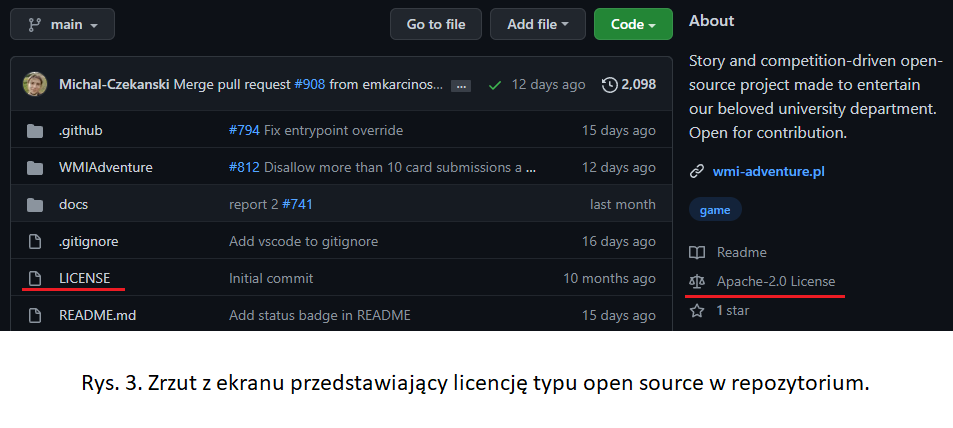
\includegraphics[width = 1\textwidth]{licencja.png}
\end{center}

\subsubsection{Dokument README}

\hspace{4mm} Plik \textbf{README} wyjaśnia jak korzystać z projektu, jakie ma on znaczenie oraz co użytkownicy mogą z nim zrobić. Taki dokument powinien odpowiadać na pytania\cite{opensource.guide}:
\begin{itemize}
    \item Co robi projekt?
    \item Dlaczego ten program jest przydatny?
    \item Jak zacząć korzystać?
    \item Gdzie jest możliwość uzyskania dodatkowej pomocy, jeśli jest ona potrzebna?
\end{itemize}

Przykładowo dokument \textbf{README} WMI Adventure, który jest dostępny pod linkiem \emph{https://github.com/emkarcinos/WMIAdventure/blob/main/README.md}\cite{wmi.readme} składa się z następujących sekcji:
\begin{enumerate}
    \item \textbf{Tytuł projektu}, a pod nim krótki opis.
    \item \textbf{Instalacja i używanie} - informacje o tym jak uruchomić aplikację oraz środowisko deweloperskie\footnote{\, Uruchomienie oprogramowania na swoim serwerze lokalnym wraz z programami ułatwiającymi zarządzanie kodem źródłowym.}.
    \item \textbf{Użyte technologie} - wymienienie stosowanych zewnętrznych modułów open source.
    \item \textbf{Wkład w rozwój} - krótka instrukcja z czym się zapoznać, aby włożyć swój wkład w rozwój projektu.
    \item \textbf{Autorzy} - wymienienie twórców aplikacji.
    \item \textbf{Licencja} - wskazanie stosowanej licencji OS.
\end{enumerate}

\subsubsection{Warunki kontrybucji}

\hspace{4mm} Plik \textbf{CONTRIBUTING} opisuje w jaki sposób można rozwijać nasze oprogramowanie OS o kolejne funkcjonalności lub wprowadzać poprawki. Warunki kontrybucji powinny być napisane tak, aby czytelnik, który jest zainteresowany pracą nad projektem uzyskał jak najwięcej wskazówek, które pomogą mu zacząć działać. W przypadku WMI Adventure opisane jest to w następujący sposób:
\begin{enumerate}
    \item Krótki opis co należy w pierwszej kolejności zrobić jeśli chcemy przyczynić się do rozwoju aplikacji.
    \item \textbf{Tworzenie issue} - opis w jaki sposób i w jakim celu tworzyć nowe \emph{issue}\footnote{\, \textbf{Issue} to funkcja serwisu \emph{GitHub}, pozwalająca dyskutować o danym zagadnieniu.}.
    \item \textbf{Implementacja własnych zmian za pomocą pull request} -\newline przedstawienie wymagań dotyczących kodu wchodzących w skład nowego \emph{pull request}\footnote{\, \textbf{Pull request} to funkcja serwisu \emph{GitHub} pozwalająca zarządzać modyfikacjami kodu, które można zaakceptować lub odrzucić.}, który zawiera zmodyfikowany kod źródłowy.
    \item \textbf{Wygląd commit'ów} - opis co powinna zawierać treść nazwy \emph{commit'a}\footnote{\, \textbf{Commit} to funkcja oprogramowania \textbf{Git} (rozproszony system kontroli wersji stworzony przez Linus'a Torvalds'a\cite{git.wiki}), która przedstawia modyfikację plików.}.
    \item \textbf{Wygląd nowego p. r.} - informacja co powinien wyrażać tytuł oraz co napisać w opisie nowego \emph{pull request'a}.
    \item \textbf{Proces akceptacji p. r.} - wymienienie kroków, które są podejmowane w celu akceptacji \emph{pull request'a}.
\end{enumerate}

\subsubsection{Kodeks postępowania}

\hspace{4mm} Dokument \textbf{CODE\_OF\_CONDUCT} pomaga ustalić podstawowe zasady postępowania dla uczestników projektu. Jest to szczególnie cenne podczas uruchamiania przedsięwzięcia OS dla społeczności lub firmy. Kodeks postępowania umożliwia autorom zdrowie ograniczając stres oraz konstruktywne zachowanie społeczności\cite{opensource.guide}. Jest możliwość zaadoptowania standardowego kodeksu ze strony pod adresem \emph{"https://www.contributor-covenant.org/"}\cite{contributor.covenant}.

\subsection{Idea społeczna open source}

\hspace{4mm} WMI Adventure jest projektem, który powstał, aby zacieśnić więzi społeczności wydziału Matematyki i Informatyki Uniwersytetu im. Adama Mickiewicza w Poznaniu. Interakcja z innymi ludźmi to jedna z najcenniejszych wartości koncepcji open source. Cytując pewnego programistę; "\texttt{Jedna z najbardziej wartościowych rzeczy, której doświadczyłem jako kontrybutor open\newline source, to relacje, które zbudowałem rozwiązując problemy razem z\newline innymi programistami}"\cite{kentcdodds}. 

Studia to również dobre środowisko do poznawania nowych osób, poprzez wspólną naukę lub wymianę poglądów. WMI Adventure w pewien sposób ma łączyć społeczne aspekty open source ze studencką integracją. Podczas kształcenia się w środowisku publicznym, napotykamy wiele pojęć oraz sytuacji, które zapadają nam nostalgicznie w pamięć. Poprzez aplikację WMI Adventure dzielimy się tymi przeżyciami, ponieważ polega ona na manipulowaniu treścią wirtualnych kart, które przeznaczone są do pojedynkowania się pomiędzy użytkownikami. Nie tylko kod źródłowy jest open source, ale również sama zawartość oprogramowania, ponieważ może ona być dowolnie dodawana oraz modyfikowana, co zapewnia nieograniczone możliwości.

Aplikacja ma potencjał, aby być dalej rozwijana przez kolejne pokolenia studentów lub innych miłośników informatyki, którzy będą chętni do przekazania swoich własnych naukowych doświadczeń zarówno za pomocą kodu źródłowego jak i treści nawiązujących do informatycznych przygód.

\newpage
\begin{thebibliography}{99}
\bibitem{Kotula}
    Sebastian Dawid Kotuła, \emph{Wstęp do Open Source}
\bibitem{Richter}
  Richter Susanne, \emph{Critique for the open source development model}, München 2007.
\bibitem{opensource.org}
  \emph{The open source definition (annotated)} [online], [dostęp: 24.11.2021]. Dostępny w WWW: http://www.opensource.org/osd.html.
\bibitem{wikipedia1}
  \emph{Licencja oprogramowania} [online], [dostęp: 24.11.2021]. Dostępny w WWW: https://pl.wikipedia.org/wiki/Licencja\_oprogramowania.
\bibitem{wikipedia2}
  \emph{GNU General Public License} [online], [dostęp: 24.11.2021]. Dostęp: https://pl.wikipedia.org/wiki/GNU\_General\_Public\_License
\bibitem{wikipedia3}
  \emph{Licencje BSD} [online], [dostęp: 25.11.2021]. Dostęp: https://pl.wikipedia.org/wiki/Licencje\_BSD
\bibitem{sjp}
  \emph{Znaczenie terminu copyright} [online], [dostęp: 25.11.2021] https://sjp.pwn.pl/slowniki/copyright.html.
\bibitem{gnu.manifest}
  Richard Stallman, \emph{Manifest GNU} [online], [dostęp: 27.11.2021]. Dostępny w WWW: https://www.gnu.org/gnu/manifesto.pl.html.
\bibitem{Webbink}
  Mark H Webbink, Red Hat, Inc., \emph{Understanding Open Source Software}
\bibitem{gnu.free}
  Free Software Foundation, \emph{Co to wolne oprogramowanie?} [online], [dostęp: 29.11.2021]. Dostępny na https://www.gnu.org/philosophy/free-sw.html.
\bibitem{gnu.difference}
  Richard Stallman, \emph{Dlaczego otwartemu oprogramowaniu umyka idea Wolnego Oprogramowania} [online], [dostęp: 29.11.2021]. Dostępny na https://www.gnu.org/philosophy/open-source-misses-the-point.html.
\bibitem{microsoft.edge}
  Surur, \emph{Microsoft wspiera projekt Chromium} [online], [dostęp: 9.12.2021]. Autorstwa "Surur" https://mspoweruser.com/author/surur/. 
  Dostęp na https://mspoweruser.com/microsoft-touts-their-contributions-to-chromium-development/.
\bibitem{vscode.mit}
    Chris Dias, \emph{Licencja VS code} [online], [dostęp: 25.12.2021].
    Dostęp na https://github.com/microsoft/vscode/blob/main/LICENSE.txt.
\bibitem{vscode.microsoft}
    \emph{Licencja Visual Studio Code jako produktu Microsoft} [online], [dostęp: 26.12.2021].
    Dostęp: https://code.visualstudio.com/license.
\bibitem{vscode.issues}
    Chris Dias, \emph{Wyjaśnienie licencjonowania Visual Studio Code w sekcji "issues" na github} [online], [dostęp: 25.12.2021].
    Dostęp: https://github.com/microsoft/vscode/issues/60.    
\bibitem{vscodium.article}
    Alan Jones, \emph{Artykuł o VSCodium} [online], [dostęp: 2.01.2022].
    Dostęp: https://towardsdatascience.com/what-is-vscodium-and-should-you-be-using-it-926e1369169a.
\bibitem{vscodium.website}
    \emph{Strona VSCodium} [online], [dostęp: 2.01.2022].
    Dostęp: https://vscodium.com/.
\bibitem{cms}
    Przemysław Durał, \emph{Co to jest CMS?} [online], [dostęp: 2.01.2022].
    Dostęp: https://ks.pl/slownik/co-to-jest-cms.    
\bibitem{wordpress.license}
    \emph{Licencja do systemu WordPress} [online], [dostęp: 2.01.2022].
    Dostęp: https://wordpress.org/about/license/.      
\bibitem{wordpress.commercial}
    \emph{Płatne dodatki do systemu WordPress} [online], [dostęp: 2.01.2022].
    Dostęp: https://wordpress.org/themes/commercial/.      
\bibitem{wiki.freeware}
    \emph{Co to jest "freeware"?} [online], [dostęp: 2.01.2022].
    Dostęp: https://en.wikipedia.org/wiki/Freeware.    
\bibitem{opensource.guide}
    \emph{Rozpoczęcie projektu Open Source} [online], [dostęp: 4.01.2022].
    Dostęp: https://opensource.guide/pl/starting-a-project/\#co-i-dlaczego-oprogramowania-typu-open-source.
\bibitem{docker.update}
    Scott Johnston, \emph{Docker is Updating and Extending Our Product Subscriptions} [online], [dostęp: 4.01.2021].
    Dostęp: https://www.docker.com/blog/updating-product-subscriptions/.    
\bibitem{docker.moby}
    \emph{What is Moby?} [online], [dostęp: 4.01.2022].
    Dostęp: https://mobyproject.org/.      
\bibitem{docker.oro}
    David Oro, \emph{Looking for a Docker Alternative? Consider This} [online], [dostęp: 4.01.2021].
    Dostęp: https://www.docker.com/blog/looking-for-a-docker-alternative-consider-this/. 
\bibitem{docker.licensing}
    \emph{Open source components and licensing} [online], [dostęp: 4.01.2022].
    Dostęp: https://docker-docs.netlify.app/docker-for-windows/opensource/. 
\bibitem{apache}
    \emph{Apache License} [online], [dostęp: 4.01.2022].
    Dostęp: https://pl.wikipedia.org/wiki/Apache\_License. 
\bibitem{wmi.readme}
    \emph{Plik README.md} [online], [dostęp: 4.01.2022].
    Dostęp: https://github.com/emkarcinos/WMIAdventure/blob/main/README.md. 
\bibitem{kentcdodds}
    Kent C. Dodds, \emph{How getting into Open Source has been awesome for me} [online], [dostęp: 5.01.2022]
    Dostęp: https://kentcdodds.com/blog/how-getting-into-open-source-has-been-awesome-for-me.
\bibitem{git.wiki}
    \emph{Git (oprogramowanie)} [online], [dostęp: 6.01.2022]
    Dostęp: https://pl.wikipedia.org/wiki/Git\_(oprogramowanie).
\bibitem{contributor.covenant}
    Coraline Ada Ehmke, \emph{A Code of Conduct for Open Source Communities} [online], [dostęp: 6.01.2022]
    Dostęp: https://www.contributor-covenant.org/.
\bibitem{elastic.def}
    \emph{Open Source Search: The Creators of Elasticsearch, ELK Stack \& Kibana} [online], [dostęp: 6.01.2022]
    Dostęp: https://www.elastic.co/.
\bibitem{elastic.license}
    \emph{Elastic License} [online], [dostęp: 6.01.2022]
    Dostęp: https://www.elastic.co/licensing/elastic-license.
\bibitem{sspl.wiki}
    \emph{Server Side Public License} [online], [dostęp: 6.01.2022]
    Dostęp: https://en.wikipedia.org/wiki/Server\_Side\_Public\_License.
\bibitem{linux.polska}
    Linux Polska, \emph{Zmiany w licencjonowaniu Elasticsearch i Kibana} [online], [dostęp: 6.01.2022]
    Dostęp: https://linuxpolska.pl/aktualnosci/zmiany-w-licencjonowaniu-elasticsearch-i-kibana/.    
    
    
\end{thebibliography}
\end{document}
